%!TEX root = ../main.tex

\chapter{Future updates, trivia and conclusions}
\label{chp:conclusions}

\section{Needed work and future updates}
\label{chp:neededWork}
\noindent
The project is far from finished and requires additional work. The following paragraphs will outline the major updates needed.

\paragraph{Security}
There are significant security vulnerabilities, particularly in the backend, which currently lacks any form of protection. It needs a system for user authentication and token creation for both the \ac{VR} app and the web app.
Additionally, the \ac{VR} app will require a user-friendly authentication interface that enables end users to authenticate themselves without difficulty.

\paragraph{Feedbacks}
Due to the limited availability of surgeons, doctors, and nurses, we were unable to conduct a thorough feedback session in which they could test the new app. Completing this step will be essential for creating a strong user experience.

\paragraph{Ready for the store}
The app is far from being ready for the Meta Quest store. Therefore, it will be necessary to comply with the store rules for publishing the app.

\paragraph{Support for new devices}
At the time of writing, Meta has also released two new devices, the Meta Quest 3 and 3s. Although they use the same \ac{OS}, it will be necessary to conduct testing to verify compatibility with these devices.

\paragraph{Future features}
The app needs to be updated for new version of Meta OS, and the app could benefit from some other functionality like:

\begin{itemize}
  \item Online multiplayer
  \item	Slicing 3D models
  \item Procedural \ac{LOD} for 3D models
  \item	3D models caching 
  \item	New environments
\end{itemize}

\section{Science4All}
\noindent
Science4All is a science outreach and inclusion project in Padua, aimed at making complex scientific topics accessible to a broad audience,
from young people to adults without a scientific background, with particular attention to people with disabilities or from disadvantaged backgrounds.\\
For the occasion, the \ac{VR} app was presented in the 3D printing section focused on medical applications. In a specially designed environment Fig.[\ref{fig:science4all}], we allowed children to try the \ac{HMD}, for many, it was their first time experiencing \ac{VR}. They had the opportunity to view a heart model, exploring both the exterior and interior in detail.
Both children and parents were captivated by the app capabilities and the medical use case for which it was developed.

\begin{figure}[ht]
  \centering
  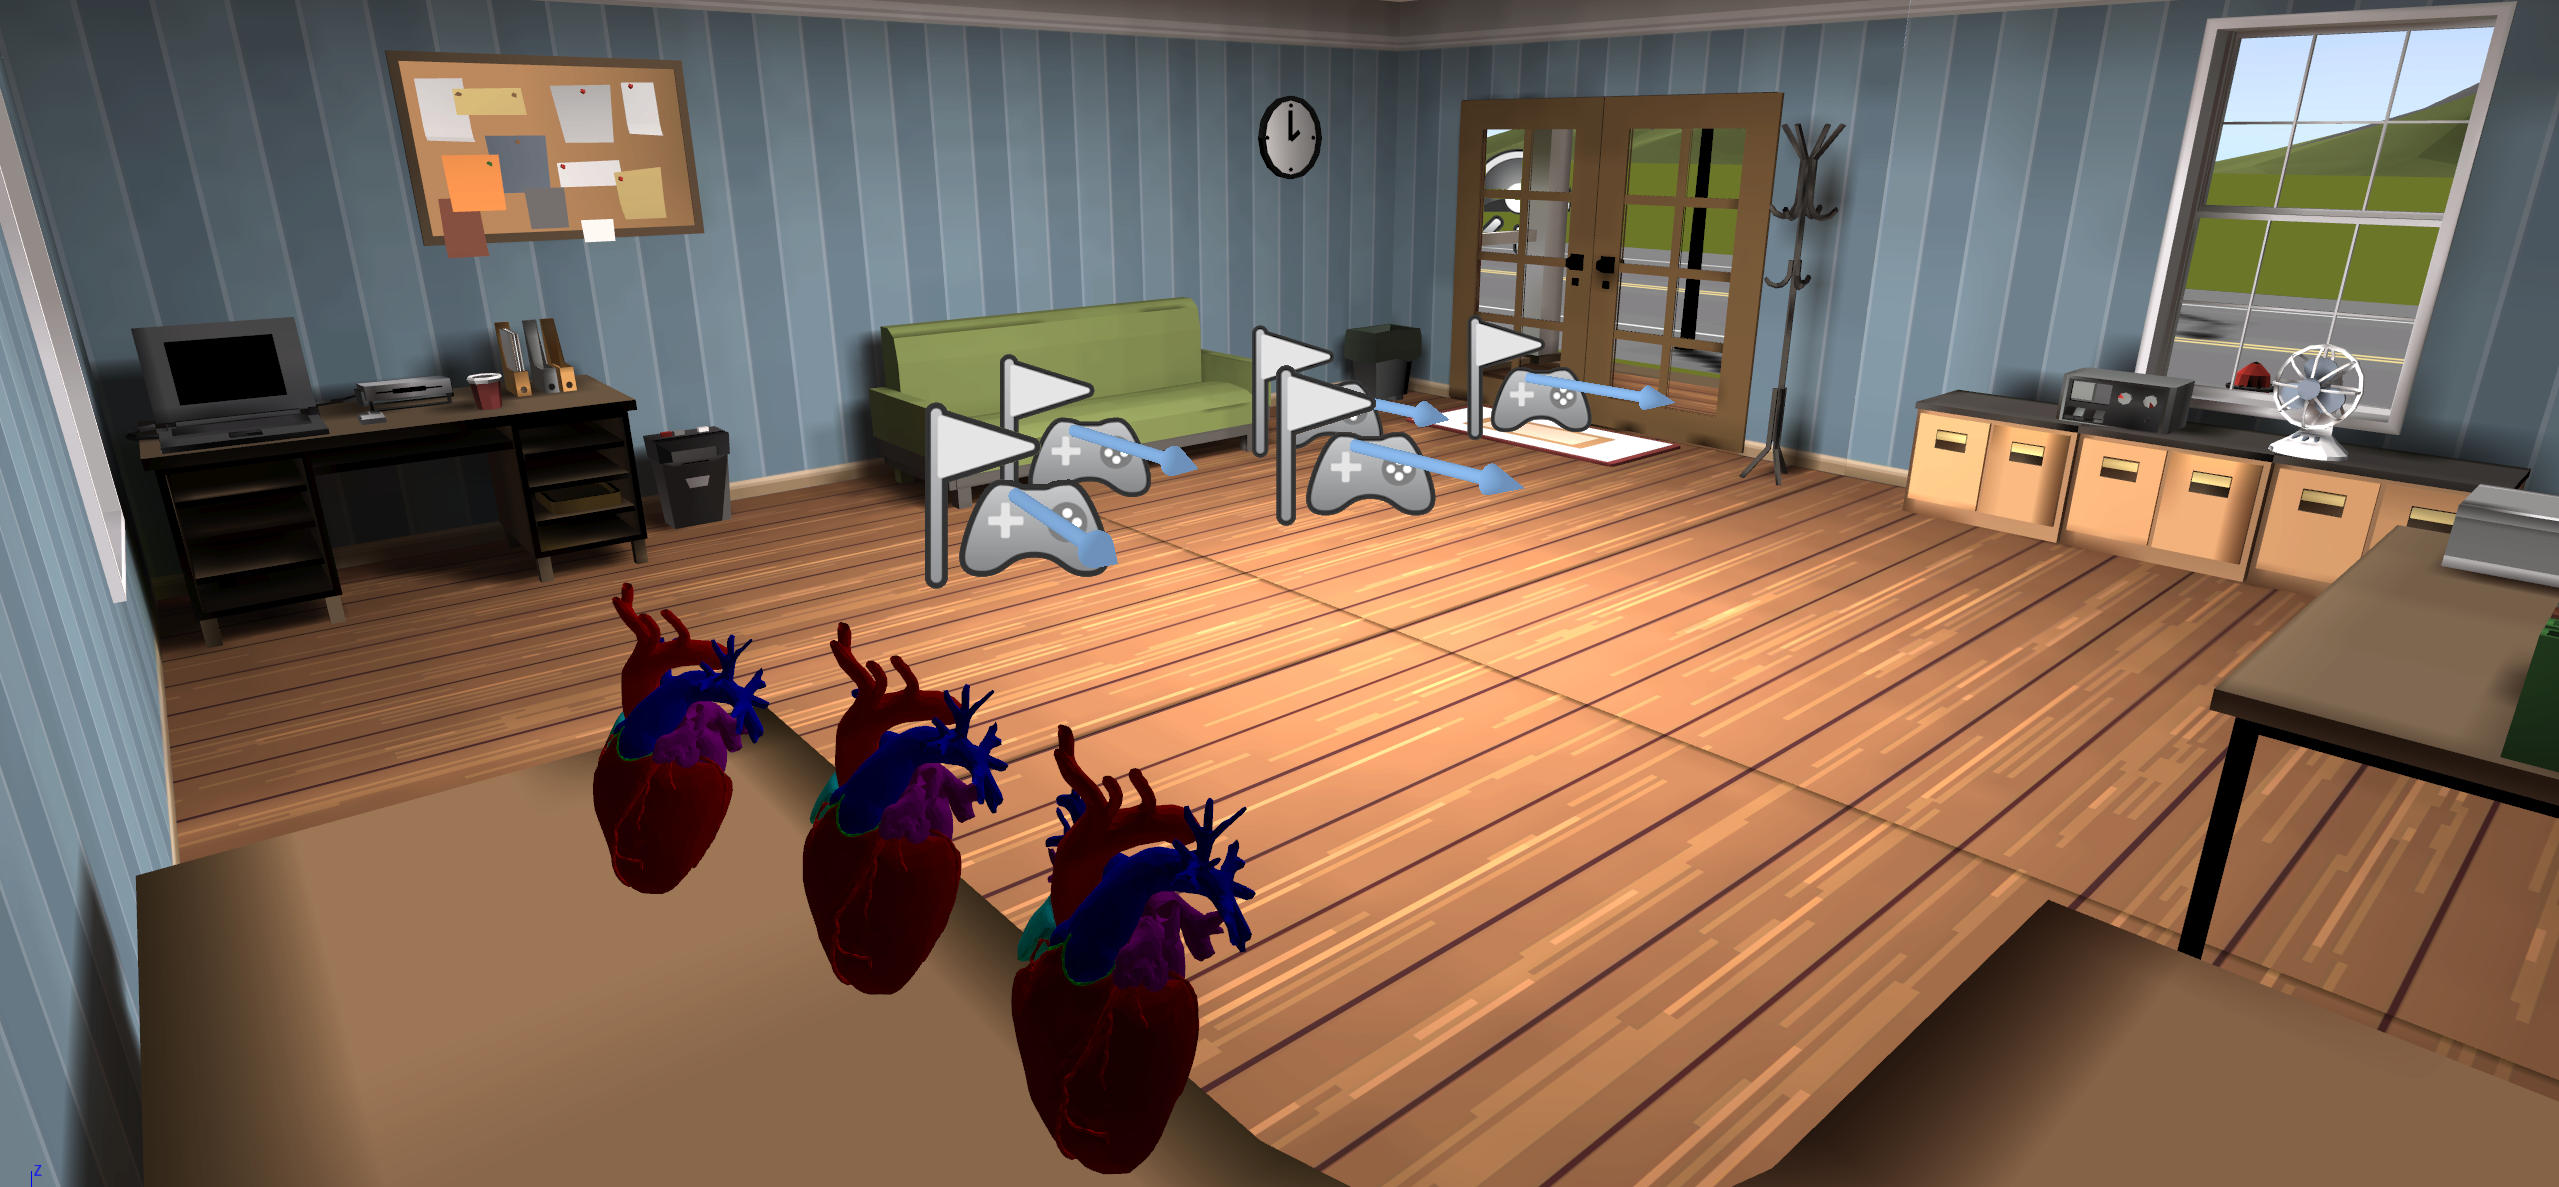
\includegraphics[width=\textwidth]{vrScreenshot/science4all.png}
  \caption{Science4All environment}
  \label{fig:science4all}
\end{figure}

\section{Conclusions}
\noindent
The development of the \ac{VR} app enabled us to create an immersive training experience for cardiac surgeons.
However, the process was challenging due to long development cycles, primarily caused by the need to compile \ac{APK} files for testing on the \ac{HMD}.\\
The project not only represent an application of the \ac{VR} technology, but also the features  that the \ac{UE} has in developing not only \ac{VR} applications but also in general 3D applications.\\
As explained in Chp.[\ref{chp:neededWork}] the project is far for finished but it is an opportunity for the university of Padua  for crating a unique application for teaching.\\